\section{Teorema de Stokes. Teorema de la divergencia de Gauss}


\subsection{Teorema de Stokes}

\begin{definición} [Rotacional]
    Sean $A \subset \mathbb{R}^3$ un conjunto abierto y $\vec{F} : A \to \mathbb{R}^3$ un campo vectorial de clase $C^1$. Se define el rotacional de $\vec{F} = (F_1,F_2,F_3)$ como:
    $$ rot(\vec{F}) = \nabla \times \vec{F} = \begin{vmatrix}
        \vec{e}_1 & \vec{e}_2 & \vec{e}_3 \\
        \frac{\partial}{\partial x} & \frac{\partial}{\partial y} & \frac{\partial}{\partial z} \\
        F_1 & F_2 & F_3
        \end{vmatrix} = \left( \frac{\partial F_3}{\partial y} - \frac{\partial F_2}{\partial z}, \frac{\partial F_1}{\partial z} - \frac{\partial F_3}{\partial x}, \frac{\partial F_2}{\partial x} - \frac{\partial F_1}{\partial y} \right)
    $$
\end{definición}

\begin{observación}
    En este caso, $rot(\vec{F})$ es un campo vectorial continuo definido en $A$.
\end{observación}

\ejemplo{
    Sea $(P,Q) : U \to \mathbb{R}^2$ un campo vectorial de clase $C^1$ definido en un abierto $U \subset \mathbb{R}^2$. Consideramos $A = U \times \mathbb{R}$ y el campo vectorial $\vec{F} = (P,Q,0)$. Entonces el rotacional de $\vec{F}$ es:
    $$ \nabla \times \vec{F} = \begin{vmatrix}
        \vec{e}_1 & \vec{e}_2 & \vec{e}_3 \\
        \frac{\partial}{\partial x} & \frac{\partial}{\partial y} & \frac{\partial}{\partial z} \\
        P & Q & 0
    \end{vmatrix} = \left( 0, 0, \frac{\partial Q}{\partial x} - \frac{\partial P}{\partial y} \right) \qquad \text{"la derivación del toerema de Green"}$$
}

\begin{teorema} [Teorema de Stokes]
    Sea $(S, \vec{n})$ una superficie orientada y regular a trozos, y sea $\vec{F}$ un campo vectorial de clase $C^1$ definido en un abierto $U \supset S$. Entonces se cumple la siguiente igualdad:
    $$ \int_{(S, \vec{n})} rot(\vec{F}) = \int_{\partial S} \vec{F} $$
    donde $\partial S$ tiene la orientación inducida por $\vec{n}$.
\end{teorema}

\ejemplo{
    Sea la superficie $S = \{(x,y,z) \in \mathbb{R}^3 : z = x^2 + y^2 \leq 4\}$ con la norma exterior $\vec{n}$ y el campo vectorial $\vec{F} = (yz, -xz, z)$. Verificamos el teorema de Stokes.\\
    Tenemos que $\partial S = \{(x,y,z) \in \mathbb{R}^3 : z = x^2 + y^2 = 4\}$, que es una circunferencia de radio $2$ en el plano $z=4$. Fijémonos que $\vec{n}$ induce la orientación negativa en la curva $C^- = \partial S$.
    \begin{center}
        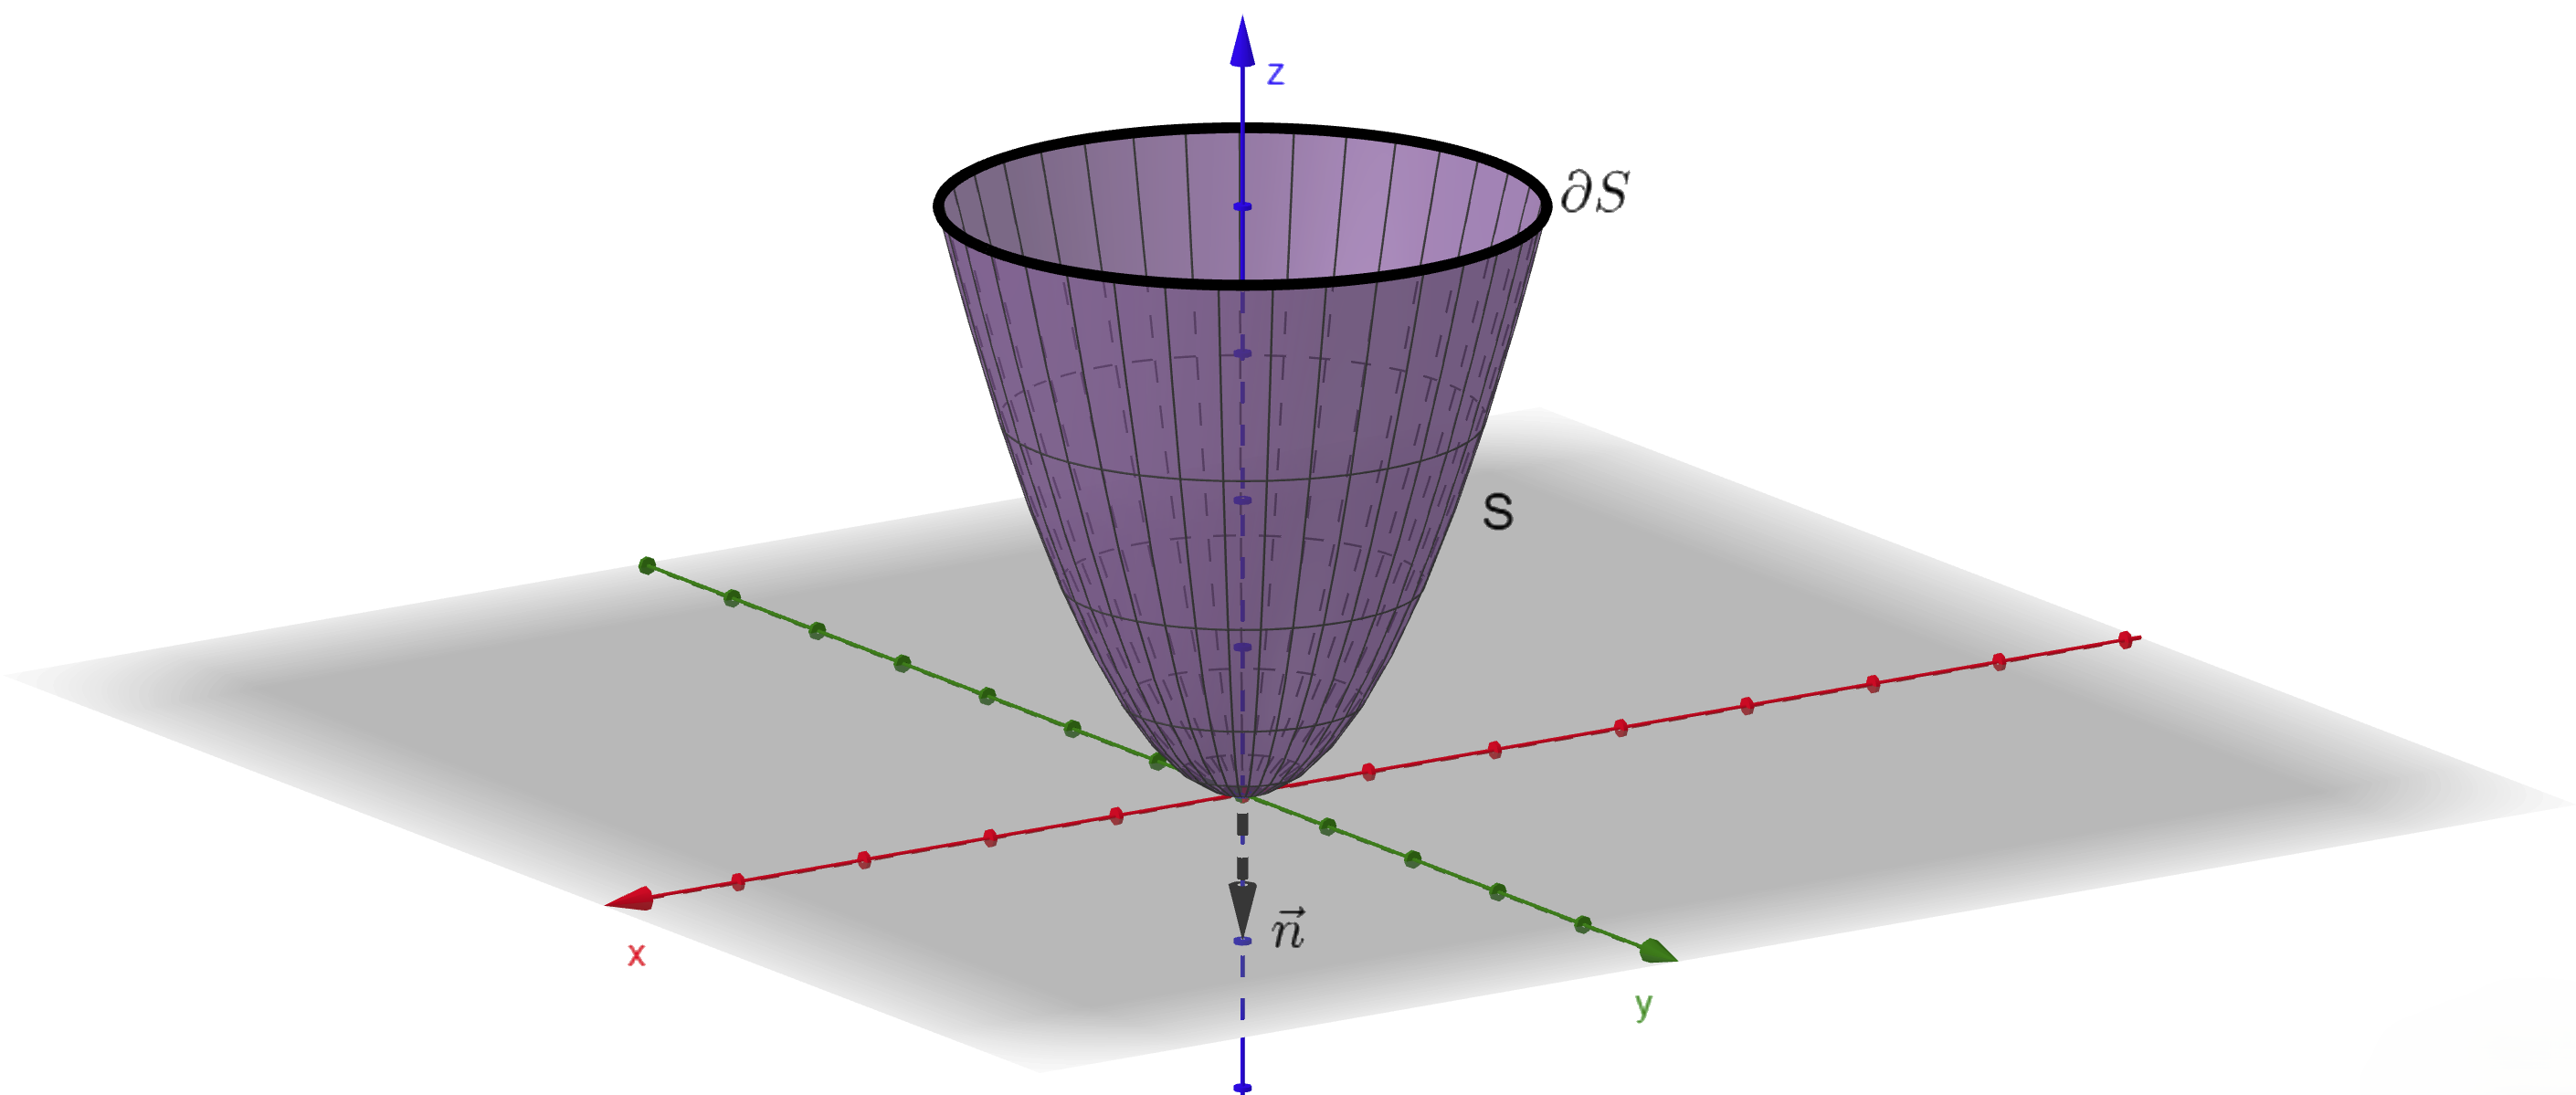
\includegraphics[width=0.65\linewidth]{images/ej4.png}
    \end{center}   
    El rotacional de $\vec{F}$ es:
    $$ rot(\vec{F}) = \nabla \times \vec{F} = \begin{vmatrix}
        \vec{e}_1 & \vec{e}_2 & \vec{e}_3 \\
        \frac{\partial}{\partial x} & \frac{\partial}{\partial y} & \frac{\partial}{\partial z} \\
        yz & -xz & z
    \end{vmatrix} = \left( x, y, -2z \right)$$
    Consideramos la parametrización natural $\varphi : D \to S$ de $S$ dada por:
    $$ \varphi(x,y) = \begin{cases}
        x = x \\
        y = y \\
        z = x^2 + y^2
    \end{cases} \qquad \text{donde } D = \{(x,y) \in \mathbb{R}^2 : x^2 + y^2 \leq 4\}$$
    Entonces la normal a la superficie $S$ es:
    $$ \vec{N}_\varphi =
        \begin{vmatrix}
            \vec{e}_1 & \vec{e}_2 & \vec{e}_3 \\
            1         & 0         & 2x        \\
            0         & 1         & 2y
        \end{vmatrix} = (-2x, -2y, 1)$$
    La normal $\vec{N}_\varphi$ apunta hacia arriba en el punto $(0,0,0)$, luego tenemos una normal interior.
    \begin{itemize}
        \item Calculamos el rotacional de $\vec{F}$ en $S$ por medio de la parametrización $\varphi$:
        $$\int_{(S, \vec{n})} rot(\vec{F}) = -\int_{D} \langle \vec{N}_\varphi, rot(\vec{F}) \circ \varphi(x,y) \rangle dx dy = -\int_{D} \langle (-2x, -2y, 1), (x,y,-2(x^2+y^2) \rangle dx dy$$
        $$ = \int_{D} 2x^2 + 2y^2 + 2x^2 + 2y^2 dx dy = \int_{D} 4(x^2+y^2) dx dy = 4 \int_{\theta=0}^{\theta=2\pi} \int_{r=0}^{r=2} r^2 \cdot r \, dr \, d\theta$$ 
        $$= 4 \cdot 2\pi \left[ \frac{r^4}{4} \right]_{r=0}^{r=2} = 4 \cdot 2\pi \cdot 4 = 32\pi$$
        \item Consideramos la parametrización positiva $\gamma$ de la curva $\partial S$ dada por:
        $$ \gamma(t) = \begin{cases}
            x = 2 \cos(t) \\
            y = 2 \sin(t) \\
            z = 4
        \end{cases} \qquad \text{donde } t \in [0,2\pi]$$
        y calculamos la integral de línea del campo $\vec{F}$ sobre la curva $\partial S$:
        $$\int_{\partial S} \vec{F} = \int_{C^-} \vec{F} = -\int_{\gamma} \vec{F} = -\int_{t=0}^{t=2\pi} \langle \vec{F}(\gamma(t)), \gamma'(t) \rangle dt $$
        $$= -\int_{t=0}^{t=2\pi} \langle (8 \sin(t), -8 \cos(t), 4), (-2 \sin(t), 2 \cos(t), 0) \rangle dt$$
        $$= \int_{t=0}^{t=2\pi} 16 dt = 16 \left[ t \right]_{t=0}^{t=2\pi} = 16(2\pi - 0) = 32\pi$$
    \end{itemize}
    En efecto, vemos que las integrales coinciden de acorde al teorema de Stokes.
}

\ejemplo{
    Sea $S = S_1 \cup S_2$, donde:
    $$
        S_1 = \{(x,y,z) \in \mathbb{R}^3 : x^2 + y^2 = 1, \ z \in [0,2] \}
        \qquad
        S_2 = \{(x,y,z) \in \mathbb{R}^3 : z = 2, \ x^2 + y^2 \leq 1 \}
    $$
    con la norma exterior $\vec{n}$ y el campo vectorial $\vec{F}(x,y,z) = (y,x,z)$. 
    El borde de $S$ es:
    $$ \partial S = C_0^+ = \{(x,y,z) \in \mathbb{R}^3 : x^2 + y^2 = 1, \ z = 0 \}$$
    \begin{center}
        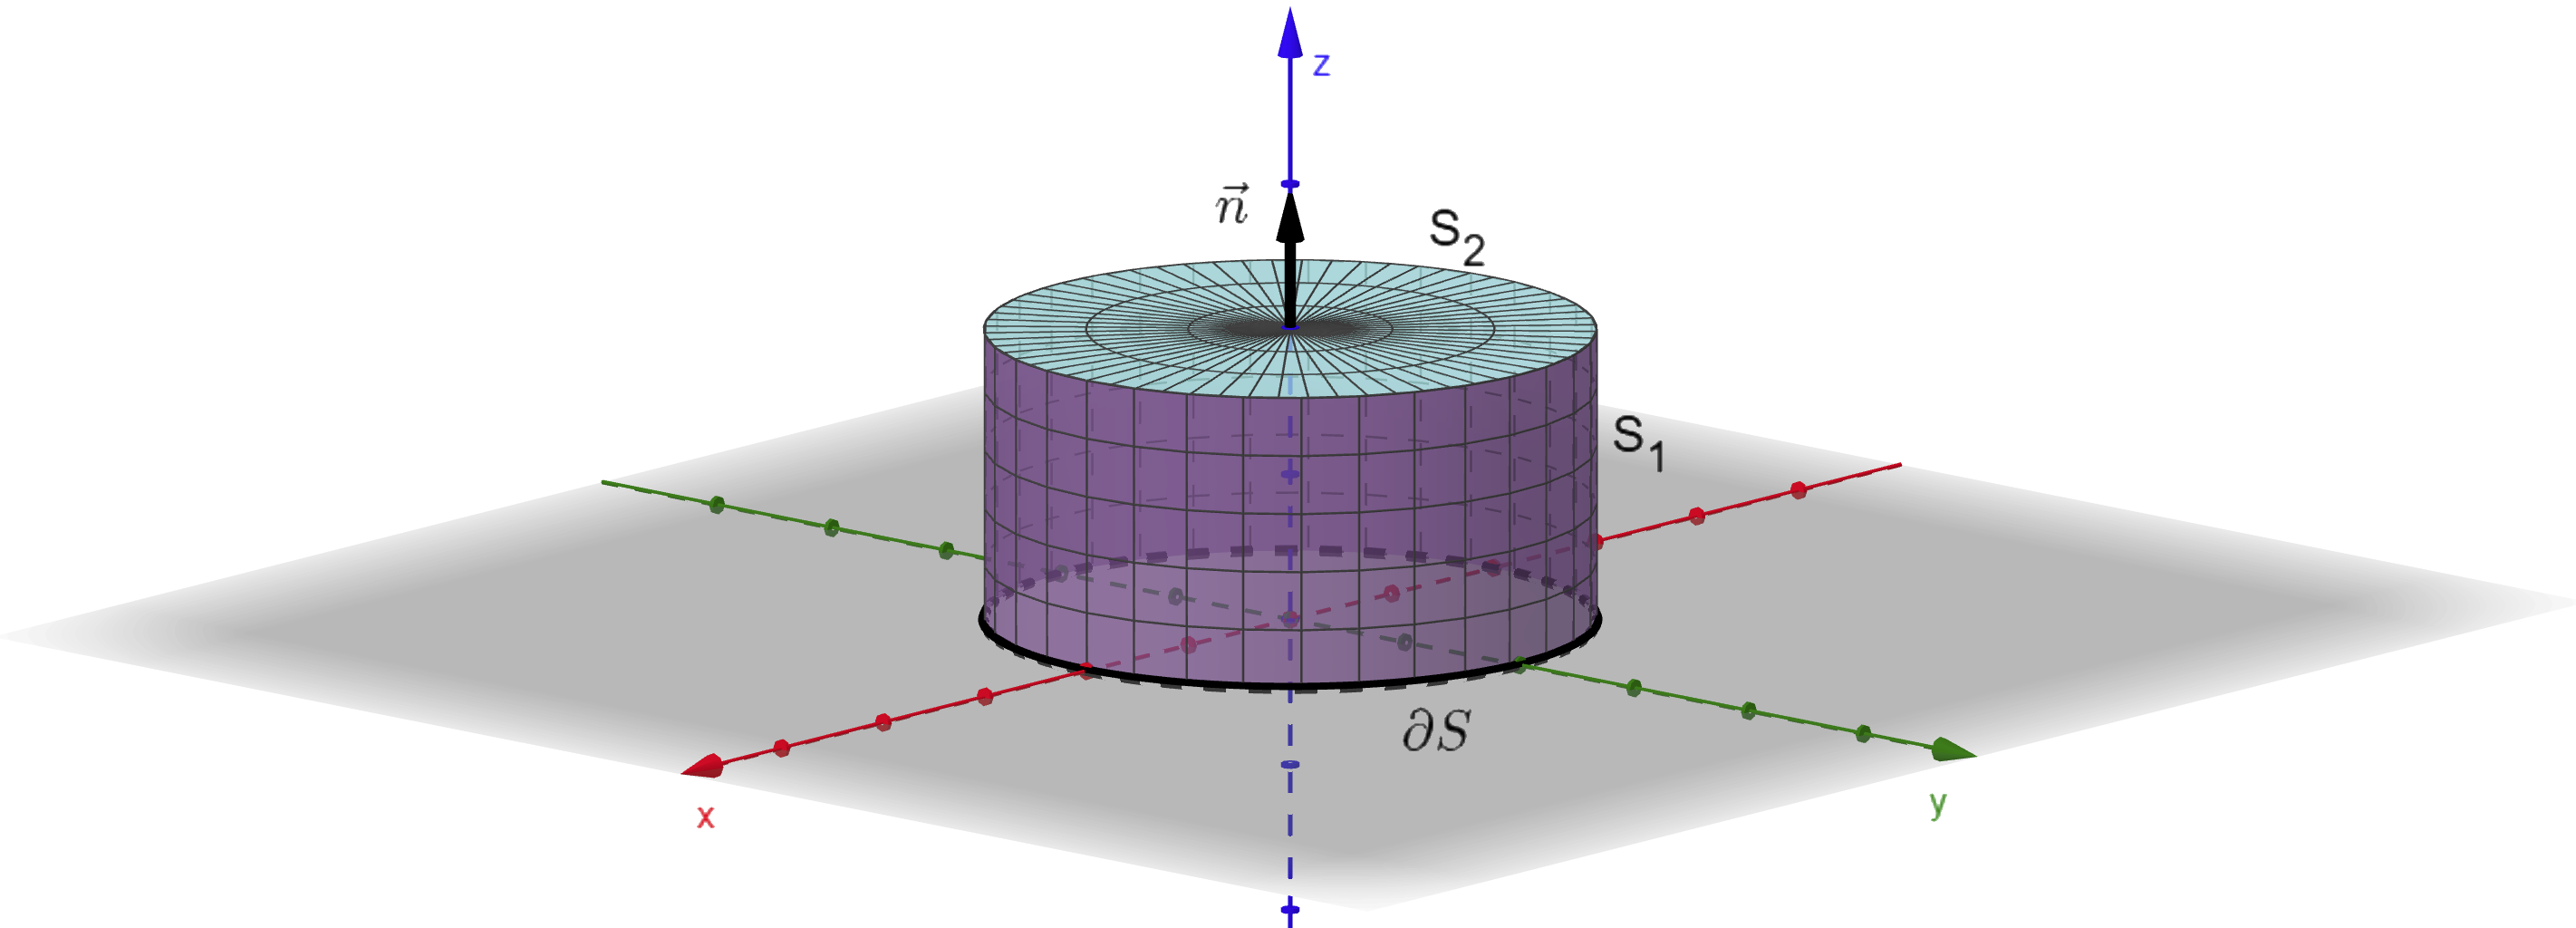
\includegraphics[width=0.65\linewidth]{images/ej5.png}
    \end{center} 
    Calculamos el rotacional del campo $\vec{F}$:
    $$ rot(\vec{F}) = \nabla \times \vec{F} = \begin{vmatrix}
        \vec{e}_1 & \vec{e}_2 & \vec{e}_3 \\
        \frac{\partial}{\partial x} & \frac{\partial}{\partial y} & \frac{\partial}{\partial z} \\
        y & x & z
    \end{vmatrix} = \left( 0, 0, 1 - 1 \right) = (0,0,0)$$
    Consideramos la parametrización $\gamma$ de la curva $C_0$ dada por:
    $$ \gamma(t) = \begin{cases}
        x = \cos(t) \\
        y = \sin(t) \\
        z = 0
    \end{cases} \qquad \text{donde } t \in [0,2\pi]$$
    que tiene orientacion positiva. Además, $\gamma'(t) = (-\sin(t), \cos(t), 0)$.
    \begin{itemize}
        \item Calculamos la integral del campo $rot(\vec{F})$ sobre la superficie $S$:
        $$\int_{(S, \vec{n})} rot(\vec{F}) = \int_{(S_1, \vec{n}_1)} \vec{0} = 0$$
        \item Hacemos la integral de línea del campo $\vec{F}$ sobre la curva $C_0^+$:
        $$\int_{\partial S} \vec{F} = \int_{C_0^+} \vec{F} = \int_{t=0}^{t=2\pi} \langle (\sin(t), \cos(t), 0), (-\sin(t), \cos(t), 0) \rangle dt$$
        $$= \int_{t=0}^{t=2\pi} \cos^2(t) - \sin^2(t) dt = \int_{t=0}^{t=2\pi} \cos(2t) dt = \left[ \frac{\sin(2t)}{2} \right]_{t=0}^{t=2\pi} = 0$$
    \end{itemize}
    Vemos que el teorema de Stokes se cumple, ya que las integrales son iguales.
}

\ejemplo{
    Consideramos el campo vectorial $\vec{F} = (yz, -xz, z)$. Veamos el rotacional de $\vec{F}$:
    $$ rot(\vec{F}) = \nabla \times \vec{F} = \begin{vmatrix}
        \vec{e}_1 & \vec{e}_2 & \vec{e}_3 \\
        \frac{\partial}{\partial x} & \frac{\partial}{\partial y} & \frac{\partial}{\partial z} \\
        yz & -xz & z
    \end{vmatrix} = \left( x, y, -2z \right)$$
    Supongamos que tenemos una superficie $S$ cualesquiera cuyo borde $\partial S$ sea la curva $C_0^+$ del ejemplo anterior. Entonces tenemos que:
    $$ \int_{(S, \vec{n})} rot(\vec{F}) = \int_{C_0^+} \vec{F} = \int_{C_0^+} \vec{F} = \int_{t=0}^{t=2\pi} \langle (0,0,0), (-\sin(t), \cos(t), 0) \rangle dt = 0$$
}

\begin{observación}
    Si $S$ es una superficie cerrada, es decir, $\partial S = \emptyset$, entonces se tiene que:
    $$ \int_{(S, \vec{n})} rot(\vec{F}) = \int_{\partial S} \vec{F} = 0$$
\end{observación}

\subsection{Geometria del Rotacional}

\ejemplo{
    Sea $\vec{F: U \to \mathbb{R}^2}$ el campo de velocidades de un fluido en $\mathbb{R}^2$. Las trayectorias son curvas $\gamma: I \to U$ con $\gamma'(t) = \vec{F}(\gamma(t))$.
}

\ejemplo{
    Sean $U \subset \mathbb{R}^3$ abierto y $\vec{F} : U \to \mathbb{R}^3$ un campo vectorial de clase $C^1$.\\
    Consideremos $p \in U$ y $r > 0$, siendo $D_r$ el circulo de centro $p$ y radio $r$, con frontera $C_r = \partial D_r$.\\
    Sea $\vec{u}$ un vector unitario de $\mathbb{R}^3$ perpendicular al plano que contiene a $D_r$, entonces:
    $$ \langle rot(\vec{F}) (p), \vec{u} \rangle = \lim_{r \to 0} \frac{1}{\pi r^2} \int_{C_r^+} \vec{F} $$
    Donde $C_r^+$ denota a $C_r$ conla orientacion comparativa a la de $\vec{u}$, y donde esta igualdad representa la "circulacion por unidad de área" del campo $\vec{F}$.   
}

\begin{proof}
    $$ \int_{C_r^+} \vec{F} = \int_{(D_r, \vec{n})} rot\vec{F} = \int_{D_r} \langle \vec{F}, \vec{u} \rangle = \int_{D_r} \langle rot\vec{F} - rot\vec{F} (p), \vec{u} \rangle + \langle rot\vec{F} (p), \vec{u} \rangle$$
    De donde pasamos a:
    $$ \int_{D_r} \langle rot\vec{F} (p), \vec{u} \rangle_{\text{constante}} = \langle rot\vec{F} (p), \vec{u} \rangle \cdot \text{área}(D_r)$$
    Entonces:
    $$ \forall \epsilon > 0, \quad \exists \delta > 0: \quad 0 < r < \delta \implies \lVert rot\vec{F} (x,y,z) - rot\vec{F} (p) \rVert < \epsilon \quad \forall (x,y,z) \in D_r \implies $$
    $$ \implies \left| \int_{D_r} \langle rot\vec{F} - rot\vec{F} (p), \vec{u} \rangle \right| \leq \int_{D_r} \left| \langle rot\vec{F} - rot\vec{F} (p), \vec{u} \rangle \right| \leq \int_{D_r} \lVert rot\vec{F} - rot\vec{F} (p) \rVert \leq \epsilon \cdot \text{área}(D_r)$$
    Luego:
    $$ \left| \frac{1}{\text{área}(D_r)} \int_{C_r^+} \vec{F} - \langle rot\vec{F} (p), \vec{u} \rangle \right| < \epsilon \quad \forall 0 < r < \delta$$
\end{proof}

\begin{definición}
    Sean $A \subset \mathbb{R}^3$ un conjunto abierto y $\vec{F} : A \to \mathbb{R}^3$ un campo vectorial de clase $C^1$. Se dice que $\vec{F}$ es irrotacional en $A$ si $rot(\vec{F}) \equiv 0$ en $A$.
\end{definición}

\begin{lema}
    Si $\vec{F}$ es un campo de clase $C^1$, y es conservativo en $A$ $\implies$ es irrotacional en $A$.
\end{lema}

\begin{proof}
    Sea $\varphi: A \to \mathbb{R}$ una función tal que $\vec{F} = \nabla \varphi$, es decir, $\vec{F} = \left( \frac{\partial \varphi}{\partial x}, \frac{\partial \varphi}{\partial y}, \frac{\partial \varphi}{\partial z} \right)$, entonces $\varphi$ es de clase $C^2$ en $A$ y, aplicando el teorema de Schwarz, tenemos que:
    $$ rot(\vec{F}) = \nabla \times \nabla \varphi = \begin{vmatrix}
        \vec{e}_1 & \vec{e}_2 & \vec{e}_3 \\
        \frac{\partial}{\partial x} & \frac{\partial}{\partial y} & \frac{\partial}{\partial z} \\
        \frac{\partial \varphi}{\partial x} & \frac{\partial \varphi}{\partial y} & \frac{\partial \varphi}{\partial z}
    \end{vmatrix} = \left( \frac{\partial^2 \varphi}{\partial y \partial z} - \frac{\partial^2 \varphi}{\partial z \partial y}, \frac{\partial^2 \varphi}{\partial z \partial x} - \frac{\partial^2 \varphi}{\partial x \partial z}, \frac{\partial^2 \varphi}{\partial x \partial y} - \frac{\partial^2 \varphi}{\partial y \partial x} \right) = (0,0,0)$$
\end{proof}

\begin{teorema}
    Sea $U \subset \mathbb{R}^3$ un abierto conexo, y sea $\vec{F} : U \to \mathbb{R}^3$ un campo vectorial de clase $C^1$. Entonces son equivalentes las siguientes afirmaciones:
    \begin{enumerate}
        \item $\vec{F}$ es conservativo en $U$.
        \item $\int_\sigma \vec{F} = 0$, $\forall \sigma$ camino triangular en $U$.
        \item $\vec{F}$ es irrotacional en $U$, es decir, $rot(\vec{F}) \equiv 0$ en $U$.
    \end{enumerate}
\end{teorema}

\begin{proof}
    \leavevmode
    \begin{itemize}
        \item (1) $\implies$ (2): Ya esta probado por la caracterizacion de los campos conservativos.
        \item (2) $\implies$ (1): Fijamos un punto $P \in U$ y consideramos para cada $x \in U$ la función
        $$ \varphi(x) = \int_{[P,x]} \vec{F}$$
        Veamos que $\varphi$ es un potencial de $\vec{F}$. Para ellos, veamos que $F_i = \frac{\partial \varphi}{\partial x_i} \ \forall i = 1,2,3$.
        $$ \lim_{h \to 0} \frac{1}{h} \left(\underbrace{\int_{[P,x + h\vec{e}_i]} \vec{F}}_{\varphi(x+h\vec{e}_i)} - \underbrace{\int_{[P,x]} \vec{F}}_{\varphi(x)} \right) = \lim_{h \to 0} \frac{1}{h} \left( \varphi(x + h\vec{e}_i) - \varphi(x) \right)$$
        Por (2), tenemos que el triangulo T de vértices $P$, $x$ y $x + h\vec{e}_i$ es tal que 
        $$\int_{[P,x] + [x,x + h\vec{e}_i] + [x + h\vec{e}_i,P]} \vec{F} = 0$$
        Luego se sigue entonces que: 
        $$ \int_{[P,x + h\vec{e}_i]} \vec{F} - \int_{[P,x]} \vec{F} = \int_{[x,x + h\vec{e}_i]} \vec{F}$$
        por tanto 
        $$\frac{1}{h} \int_{[x,x + h\vec{e}_i]} \vec{F} = \frac{1}{h} \int_{t =0}^{t=1} \langle \vec{F}(x + t h \vec{e}_i), h \vec{e}_i \rangle dt = \int_{t=0}^{t=1} \vec{F}_i(x + t h \vec{e}_i)dt \xrightarrow{h \to 0} \vec{F}_i(x)$$
        donde $\gamma(t) = x + t h \vec{e}_i$ con $t \in [0,1]$. Así obtenemos que $(1) \iff (2)$.
        \item $(3) \implies (2)$: Sea $T \subset U$ un triángulo, y sea $ \sigma = \partial T$:
        \item[] $$ \int_\sigma \vec{F} = \int_{(T, \vec{n})} rot(\vec{F}) = 0$$
    \end{itemize}
\end{proof}

\ejemplo{
    Es importante que $U$ sea convexo:\\
    Seam $U = \{(x,y,z) \in \mathbb{R}^3 : (x,y) \neq (0,0) \}$ y $\vec{F}: U \to \mathbb{R}^3$ el campo vectorial dado por:
    $$ \vec{F}(x,y,z) = \left( \frac{-y}{x^2 + y^2}, \frac{x}{x^2 + y^2}, 0 \right) = \left(P,Q,0\right)$$
    Asi tenemos el siguiente rotacional
    $$ rot(\vec{F}) = \begin{vmatrix}
        \vec{e}_1 & \vec{e}_2 & \vec{e}_3 \\
        \frac{\partial}{\partial x} & \frac{\partial}{\partial y} & \frac{\partial}{\partial z} \\
        P & Q & 0
    \end{vmatrix} = \left(0, 0, \frac{\partial Q}{\partial x} - \frac{\partial P}{\partial y}\right) = (0,0,0)$$
    El campo $\vec{F}$ es por tanto irrotacional en $U$, pero $\vec{F}$ no es conservativo. Consideremos la curva cerrada $\gamma$ dada por:
    $$ \gamma(t) = (\cos(t), \sin(t), 0), \quad t \in [0,2\pi] \implies \int_\gamma \vec{F} = \int_{t=0}^{t=2\pi} \langle \vec{F}(\gamma(t)), \gamma'(t) \rangle dt $$
    $$ = \int_{t=0}^{t=2\pi} \langle \left( \frac{-\sin(t)}{1}, \frac{\cos(t)}{1}, 0 \right), (-\sin(t), \cos(t), 0) \rangle dt = \int_{t=0}^{t=2\pi} 1 dt = 2\pi \neq 0$$
    Demostrando así que $\vec{F}$ no es conservativo.
}

\ejemplo{
    \underline{El ejercicio de Nash}:\\
    Encontrar $X \subset \mathbb{R}^3$ tal que si denotamos por 
    $$V = \{ \vec{F}: \mathbb{R}^3  \setminus X \to \mathbb{R}^3  \text{ campo } C^1 \mid rot(\vec{F}) = \vec{0} \}$$
    $$W = \{\vec{F}: \mathbb{R}^3  \setminus X \to \mathbb{R}^3  \text{ campo }C^1 \mid \vec{F} = \nabla g \text{ para algún } g \}$$
    obtengamos que $dim(V \setminus W) = 8$.
}

Sean $U \subset \mathbb{R}^3$ un abierto y $\vec{F} : U \to \mathbb{R}^3$ un campo vectorial de clase $C^1$. Recordamos que se definía la divergencia de $\vec{F}$ como:
$$ div(\vec{F}) = \nabla \cdot \vec{F} = \frac{\partial F_1}{\partial x} + \frac{\partial F_2}{\partial y} + \frac{\partial F_3}{\partial z} \quad \text{ donde } \quad \vec{F} = (F_1,F_2,F_3)$$


\begin{teorema} [Teorema de la Divergencia de Gauss]
    Sea $A \subset \mathbb{R}^3$ un conjunto abierto y acotado, y denotamos el sólido $V = \overline{A}$. Supongamos que $\partial V = S$ es una superficie cerrada, simple, regular-a-trozos y orientada con la normal exterior $\vec{n}$ a $V$.\\
    Sea $\vec{F} : U \to \mathbb{R}^3$ un campo vectorial de clase $C^1$, definido en un conjunto abierto $U \supset V$. Entonces se cumple la siguiente igualdad:
    $$ \int_{V} div(\vec{F}) = \int_{(S, \vec{n})} \vec{F} = \int_{(\partial V, \vec{n})} \vec{F}$$
\end{teorema}


\begin{proof}
    \underline{\text{Para dominios proyectables:}}\\
    Supongamos que $V$ es z-proyectable, es decir, $V = \{(x,y,z) \in \mathbb{R}^3 : (x,y) \in D, h(x,y) \leq z \leq g(x,y) \}$, donde $\overline{D} = D \cup C$ como en el teorema de Green, y $h,g : \overline{D} \to \mathbb{R}$ son funciones de clase $C^1$.
    $$\int_{V} div(\vec{F}) = \int_{V} \frac{\partial F_1}{\partial x} + \frac{\partial F_2}{\partial y} + \frac{\partial F_3}{\partial z}$$
    siendo $\vec{F} = (F_1,F_2,F_3)$.
    Veamos que 
    $$\int_{V} div(\vec{F}) = \int_{\partial V} \vec{F} = \int_{\partial V} (F_1,0,0) + \int_{\partial V} (0,F_2,0) + \int_{\partial V} (0,0,F_3)$$
    Para ellos probaremos que $\int_{V} \frac{\partial F_3}{\partial z} = \int_{\partial V} (0,0,F_3)$. Suponiendo que $V$ es además x-proyectable e y-proyectable, obtendremos los resultados análogos para las integrales de $F_1$ y $F_2$.\\
    $$\partial V = S_0 \cup S_g \cup S_h \quad \text{donde se definen las siguientes superficies:}$$
    $$S_0 = \{(x,y,z) \in \mathbb{R}^3 : (x,y) \in \partial D, h(x,y) \leq z \leq g(x,y) \}$$
    $$S_g = \{(x,y,z) \in \mathbb{R}^3 : (x,y) \in D, z = g(x,y)\}$$
    $$S_h = \{(x,y,z) \in \mathbb{R}^3 : (x,y) \in D, z = h(x,y)\}$$
    Considerando las parametrizaciones naturales $\varphi_g$ y $\varphi_h$ de $S_g$ y $S_h$, respectivamente, tenemos que:
    $$\varphi_g(x,y) = \begin{cases}
        x = x \\
        y = y \\
        z = g(x,y)
    \end{cases} \qquad \varphi_h(x,y) = \begin{cases}
        x = x \\
        y = y \\
        z = h(x,y)
    \end{cases}$$
    Entonces la normal a la superficie $S_g$ es:
    $$\vec{N}_g = \frac{\partial \varphi_g}{\partial x} \times \frac{\partial \varphi_g}{\partial y} = \begin{vmatrix}
        \vec{e}_1 & \vec{e}_2 & \vec{e}_3 \\
        1         & 0         & \frac{\partial g}{\partial x} \\
        0         & 1         & \frac{\partial g}{\partial y}
    \end{vmatrix} = \left( -\frac{\partial g}{\partial x}, -\frac{\partial g}{\partial y}, 1 \right)$$
    que es la norma exterior, pues $\vec{N}_g$ apunta hacia arriba y la superficie $S_g$ es la parte superior de $V$. Por tanto, la orientación es positiva.\\
    En el caso de $S_h$, tenemos que la normal es:
    $$\vec{N}_h = \frac{\partial \varphi_h}{\partial x} \times \frac{\partial \varphi_h}{\partial y} = \begin{vmatrix}
        \vec{e}_1 & \vec{e}_2 & \vec{e}_3 \\
        1         & 0         & \frac{\partial h}{\partial x} \\
        0         & 1         & \frac{\partial h}{\partial y}
    \end{vmatrix} = \left( -\frac{\partial h}{\partial x}, -\frac{\partial h}{\partial y}, 1 \right)$$
    que es la norma interior, pues $\vec{N}_h$ apunta hacia arriba también, pero al ser $S_h$ la parte inferior de $V$, el vector es interior. Por tanto, la orientación es negativa.\\
    En $S_0$, el vector normal $\vec{n}_0 = (n_1,n_2,0)$ es perpendicular al vector $(0,0,1)$, y por tanto se tiene que:
    $$\int_{(S_0, \vec{n}_0)} (0,0,F_3) = \int_{S_0} \langle (0,0,F_3), (n_1,n_2,0) \rangle = \int_{S_0} 0 = 0$$
    $$\int_{(\partial V, \vec{n}_0)} (0,0,F_3) = \underbrace{\int_{(S_0, \vec{n}_0)} (0,0,F_3)}_{0} + \int_{(S_g, \vec{n}_g)} (0,0,F_3) + \int_{(S_h, \vec{n}_h)} (0,0,F_3)$$
    $$= \int_{\overline{D}} \vec{F}_3(x,y,g(x,y)) - \vec{F}_3(x,y,h(x,y))dxdy$$
    por el teorema de Fubini tenemos 
    $$ = \int_{D} \left[ F_3(x,y,z) \right]_{z=h(x,y)}^{z=g(x,y)} dx dy =\int_{V} \frac{\partial F_3}{\partial z} dz dy dx$$
\end{proof}

\begin{observación}
    Aquí, $\partial V = S = Fr(V)$ es la frontera topológica de $V$.
\end{observación}

\ejemplo{
    Verficar el teorema para el siguiente dominio:
    $$ V = \{(x,y,z) \in \mathbb{R}^3 : x^2 + y^2 \leq 1, \ z \in [0,2] \}$$
    y el campo vectorial $\vec{F}(x,y,z) = (xy^2, x^2y, z)$.
    Entonces vemos que la frontera de $V$ viene dada por $\partial V = S_0 \cup S_1 \cup S_2$, donde:
    $$ S_0 = \{(x,y,z) \in \mathbb{R}^3 : x^2 + y^2 \leq 1, \ z = 0 \}$$
    $$ S_1 = \{(x,y,z) \in \mathbb{R}^3 : x^2 + y^2 = 1, \ z \in [0,2] \}$$
    $$ S_2 = \{(x,y,z) \in \mathbb{R}^3 : x^2 + y^2 \leq 1, \ z = 2 \}$$
    \begin{center}
        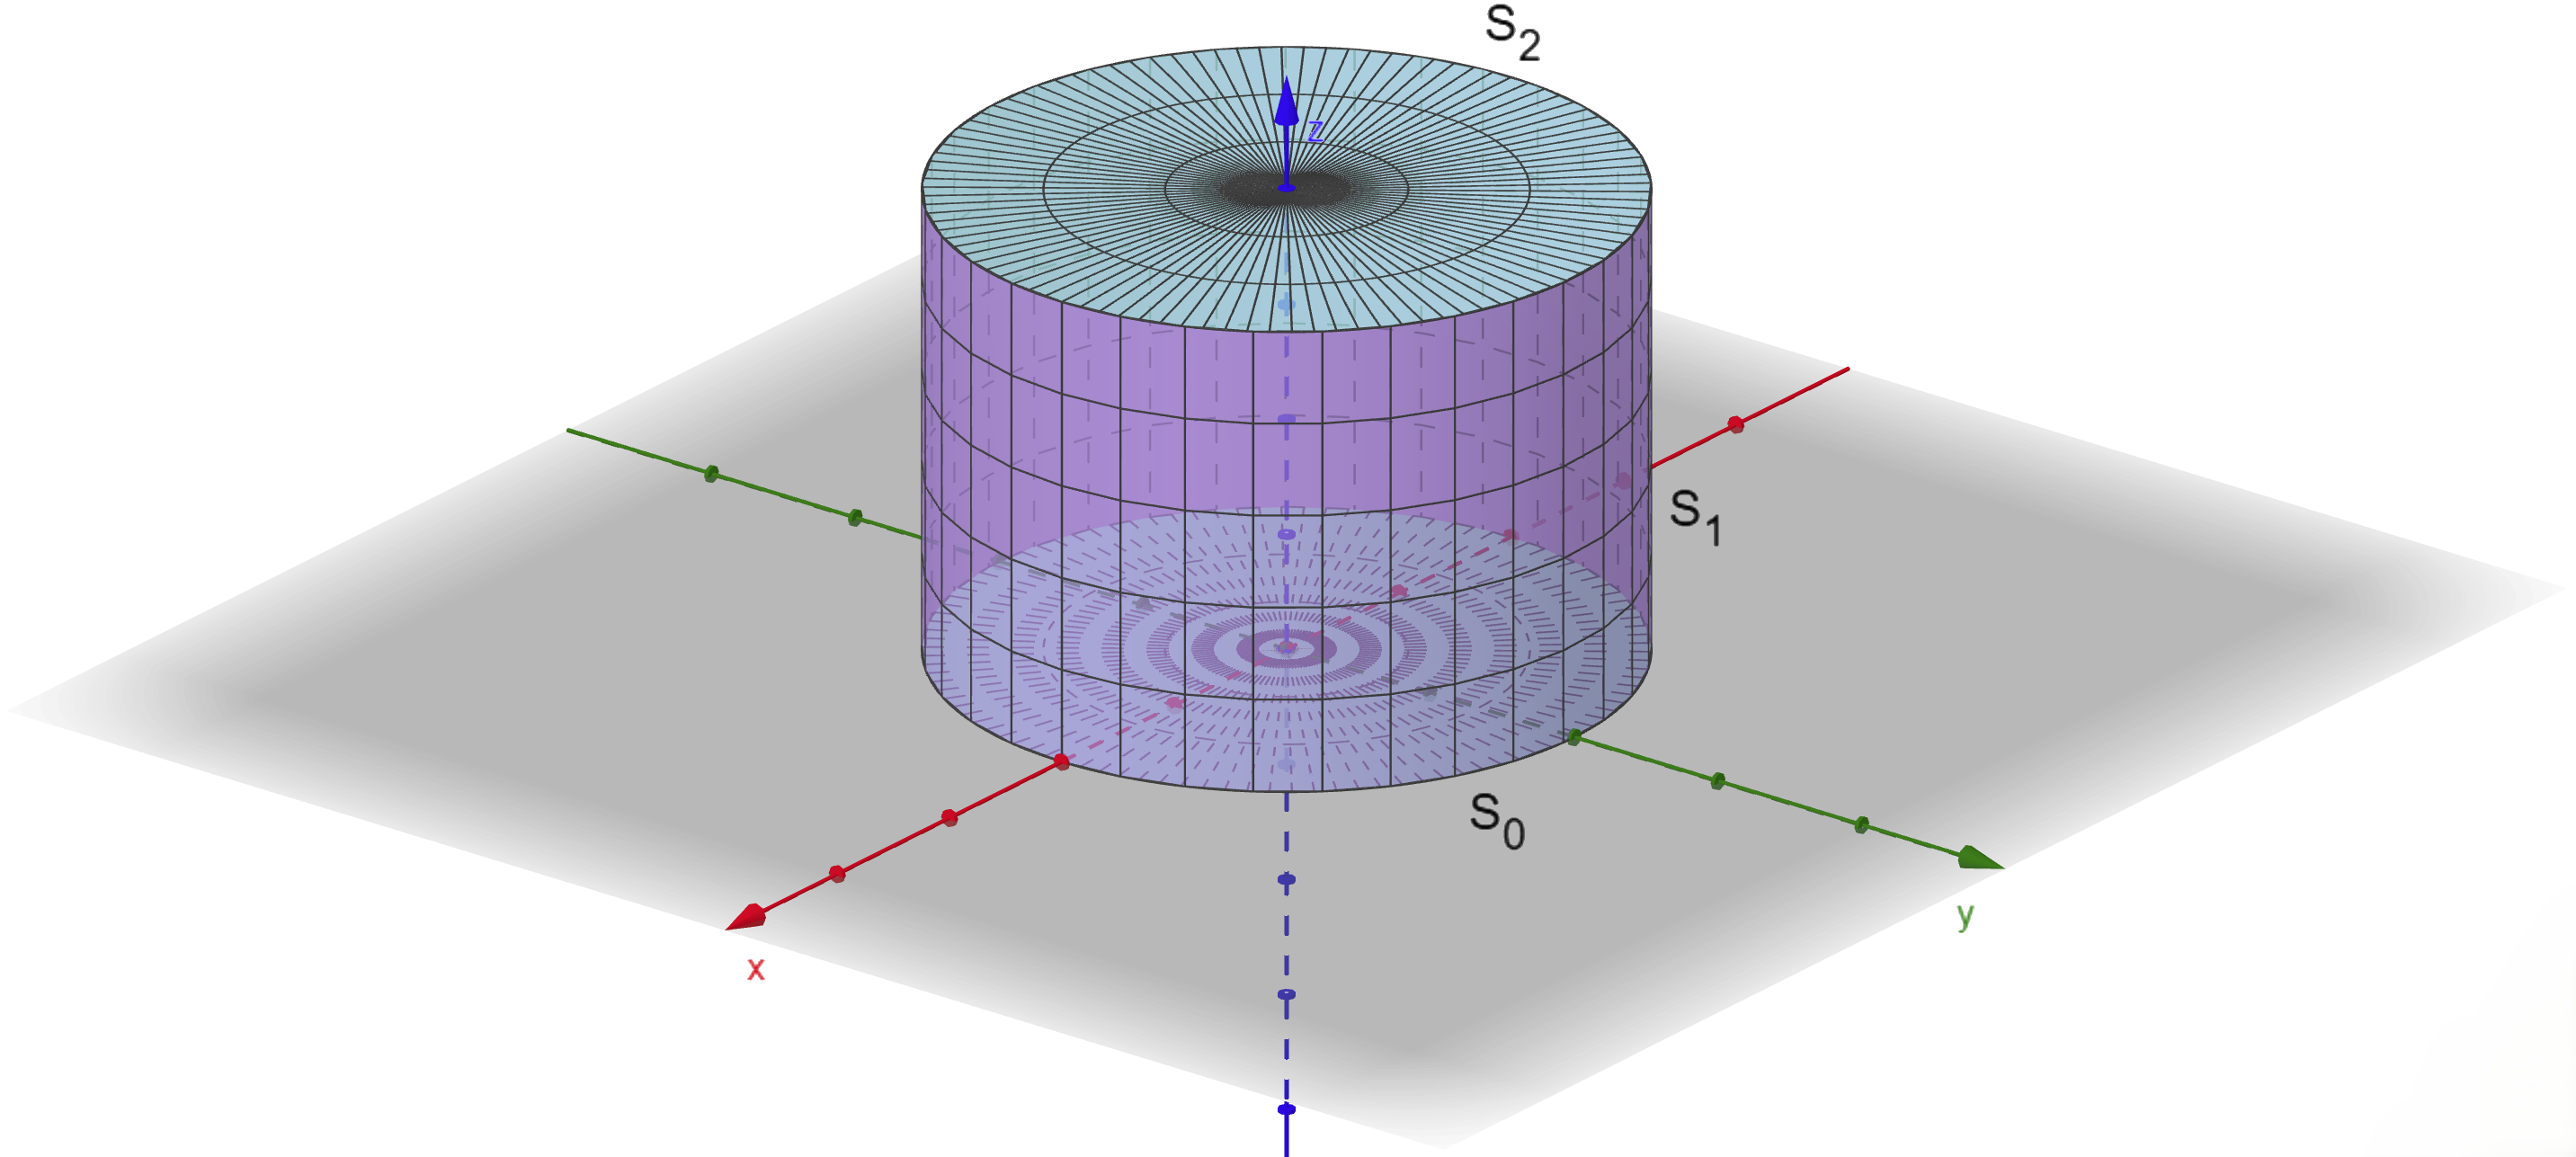
\includegraphics[width=0.5\linewidth]{images/ej6.png}
    \end{center} 
    Entonce se tiene que $div(\vec{F}) = \frac{\partial F_1}{\partial x} + \frac{\partial F_2}{\partial y} + \frac{\partial F_3}{\partial z} = y^2 + x^2 + 1$.
    \begin{itemize}
        \item $$\int_{V} div(\vec{F}) = \int_{V} (y^2 + x^2 + 1) dx dy dz = \int_{z=0}^{z=2} \int_{\theta =0}^{\theta=2\pi} \int_{r=0}^{r=1} r(r^2+1)dr d\theta dz$$
        $$= 4 \pi \int_{r=0}^{r=1} r^3+rdr = 4 \pi \left[ \frac{r^4}{4} + \frac{r^2}{2} \right]_{r=0}^{r=1} = 4\pi \left( \frac{1}{4} + \frac{1}{2} \right) = 4\pi \cdot \frac{3}{4} = 3\pi$$
        \item $$\int_{(\partial V, \vec{n})} \vec{F} = \int_{(S_0, \vec{n}_0)} \vec{F} + \int_{(S_1, \vec{n}_1)} \vec{F} + \int_{(S_2, \vec{n}_2)} \vec{F}$$
        $$S_1 \rightarrow \varphi_1(x,y) = \begin{cases}
            x = \cos(\theta) \\
            y = \sin(\theta) \\
            z = z
        \end{cases} \qquad \text{donde } \theta \in [0,2\pi], z \in [0,2]$$
        siendo $D = \{ (\theta,z) \in \mathbb{R}^2 : \theta \in [0,2\pi], z \in [0,2] \}$.
        Entonces:
        $$\vec{N}_{\varphi_1} = \begin{vmatrix}
            \vec{e}_1 & \vec{e}_2 & \vec{e}_3 \\
            -\sin(\theta) & \cos(\theta) & 0 \\
            0 & 0 & 1
        \end{vmatrix} = (\cos(\theta), \sin(\theta), 0)$$
        que es una orientacion positiva, luego se tiene que
        $$\int_{(S_1, \vec{n}_1)} \vec{F} = \int_{D} \langle \vec{F}(\varphi_1(x,y)), \vec{N}_{\varphi_1} \rangle dx dy$$ 
        $$= \int_{\theta =0}^{\theta=2\pi} \int_{z=0}^{z=2} \langle (\cos(\theta) \sin^2(\theta), \cos^2(\theta) \sin(\theta), z), (\cos(\theta), \sin(\theta), 0) \rangle dz d\theta$$
        $$= \int_{\theta =0}^{\theta=2\pi} \int_{z=0}^{z=2} 2 \cos^2(\theta) \sin^2(\theta)dz d\theta = 4 \int_{\theta =0}^{\theta=2\pi} \cos^2(\theta) (1-\cos^2(\theta)) d\theta = \pi$$
        $$S_0 \rightarrow \varphi_0(x,y) = \begin{cases}
            x = x \\
            y = y \\
            z = 0
        \end{cases} \qquad \text{donde } x^2 + y^2 \leq 1$$
        siendo $E = \{ (x,y) \in \mathbb{R}^2 : x^2 + y^2 \leq 1 \}$.
        Entonces:
        $$\vec{N}_{\varphi_0} = \begin{vmatrix}
            \vec{e}_1 & \vec{e}_2 & \vec{e}_3 \\
            1 & 0 & 0 \\
            0 & 1 & 0
        \end{vmatrix} = (0,0,1)$$
        que es una orientacion negativa, luego se tiene que
        $$\int_{(S_0, \vec{n}_0)} \vec{F} = -\int_{E} \langle \vec{F}(\varphi_0(x,y)), \vec{N}_{\varphi_0} \rangle dx dy = -\int_{E} \langle (xy^2, x^2y, 0), (0,0,1) \rangle dx dy = 0$$
        $$S_2 \rightarrow \varphi_2(x,y) = \begin{cases}
            x = x \\
            y = y \\
            z = 2
        \end{cases} \qquad \text{donde } x^2 + y^2 \leq 1$$
        siendo $E = \{ (x,y) \in \mathbb{R}^2 : x^2 + y^2 \leq 1 \}$.
        Entonces:
        $$\vec{N}_{\varphi_2} = \begin{vmatrix}
            \vec{e}_1 & \vec{e}_2 & \vec{e}_3 \\
            1 & 0 & 0 \\
            0 & 1 & 0
        \end{vmatrix} = (0,0,1)$$
        que es una orientacion positiva, luego se tiene que
        $$\int_{(S_2, \vec{n}_2)} \vec{F} = \int_{E} \langle \vec{F}(\varphi_2(x,y)), \vec{N}_{\varphi_2} \rangle dx dy = \int_{E} \langle (xy^2, x^2y, 2), (0,0,1) \rangle dx dy$$ 
        $$= 2 \int_{E} dx dy = 2area(E) = 2 \cdot \pi$$
        \item Entonces, sumando las integrales:
        $$\int_{(S_0, \vec{n}_0)} \vec{F} + \int_{(S_1, \vec{n}_1)} \vec{F} + \int_{(S_2, \vec{n}_2)} \vec{F} = 0 + \pi + 2\pi = 3\pi$$
        Vemos que las integrales coinciden, por lo que se cumple el teorema de la divergencia de Gauss.
    \end{itemize}
}

\begin{teorema} [Teorema de la Divergencia de Gauss]
    Sea $V \subset \mathbb{R}^3$ un sólido cuya frontera $S = \partial V$ es una superficie simple regular a trozos, que está orientada con la normal exterior $\vec{n}$ a $V$.\\
    Sea $\vec{F} : U \to \mathbb{R}^3$ un campo vectorial de clase $C^1$, definido en un conjunto abierto $U \supset V \cup S$. Entonces se cumple la siguiente igualdad:
    $$ \int_{V} div(\vec{F}) = \int_{(S, \vec{n})} \vec{F}$$
\end{teorema}

\underline{Geometría de la Divergencia:}\\
\begin{corolario}
    En las condiciones anteriores, para cada $p \in U$ sea $B_r(p)$ la bola de radio $r$ centrada en $p$ y denotamos $S_r(p) = \partial B_r(p)$ la esfera correspondiente orientada con la normal exterior $\vec{n}$ a $B_r(p)$. En este caso, se cumple que:
    $$ div(\vec{F})(p) = \lim_{r \to 0} \frac{1}{m(B_r(p))} \int_{(S_r(p), \vec{n})} \vec{F}$$ 
\end{corolario}

\begin{proof}
    Denotamos $f = div(\vec{F}) : U \to \mathbb{R}$ que es una función continua en $U$.\\
    Entonces $\forall \epsilon > 0$, $\exists \delta > 0$ tal que si $0 < r < \delta$ se cumple que:
    $$ \left| f(x) - f(p) \right| < \epsilon \quad \forall x \in B_r(p)$$
    Entonces, por el teorema de la divergencia de Gauss, tenemos que:
    $$ \left| f(p) - \frac{1}{m(B_r(p))} \int_{(S_r(p), \vec{n})} \vec{F} \right| = \left| f(p) - \frac{1}{m(B_r(p))} \int_{(S_r(p), \vec{n})} f(x) \right|$$
    $$ = \left| \frac{1}{m(B_r(p))} \left( \int_{B_r(p)} f(p) - \int_{(S_r(p), \vec{n})} f(x) \right) \right|$$
    $$ \leq \frac{1}{m(B_r(p))} \left| \int_{B_r(p)} \left| f(p) - f(x) \right| \right| \leq \frac{1}{m(B_r(p))} m(B_r(p)) \cdot \epsilon = \epsilon$$
\end{proof}

\begin{observación}
    Si $div(\vec{F})(p) = 0$ para todo $p \in U$, entonces se dice que $\vec{F}$ es incompresible en $U$.
\end{observación}

\begin{observación}
    Sea $\vec{F} : U \to \mathbb{R}^3$ un campo vectorial de clase $C^1$. Entonces se cumple que:
    $$ div(rot(\vec{F})) \equiv 0 \quad \text{en } U$$
\end{observación}

\begin{proof}
    $$ rot(\vec{F}) = \begin{vmatrix}
        \vec{e}_1 & \vec{e}_2 & \vec{e}_3 \\
        \frac{\partial}{\partial x} & \frac{\partial}{\partial y} & \frac{\partial}{\partial z} \\
        F_1 & F_2 & F_3
    \end{vmatrix} = \left( \frac{\partial F_3}{\partial y} - \frac{\partial F_2}{\partial z}, \frac{\partial F_1}{\partial z} - \frac{\partial F_3}{\partial x}, \frac{\partial F_2}{\partial x} - \frac{\partial F_1}{\partial y} \right)$$
    $$ div(rot(\vec{F})) = \frac{\partial^2 F_3}{\partial x \partial y} - \frac{\partial^2 F_2}{\partial x \partial z} + \frac{\partial^2 F_1}{\partial y \partial z} - \frac{\partial^2 F_3}{\partial y \partial x} + \frac{\partial^2 F_2}{\partial z \partial x} - \frac{\partial^2 F_1}{\partial z \partial y} \equiv 0$$
    por ser $\vec{F}$ de clase $C^2$.
\end{proof}

\begin{observación}
    Si $\varphi : U \to \mathbb{R}$ es una función de clase $C^2$, entonces se cumple que:
    $$ rot(\nabla \varphi) \equiv 0 \quad \text{en } U$$
\end{observación}

\begin{observación}
    Si $\varphi : U \to \mathbb{R}$ es una función de clase $C^2$, entonces se cumple que:
    $$ div(\nabla \varphi) = div\left(\frac{\partial \varphi}{\partial x}, \frac{\partial \varphi}{\partial y}, \frac{\partial \varphi}{\partial z}\right) = \frac{\partial^2 \varphi}{\partial x^2} + \frac{\partial^2 \varphi}{\partial y^2} + \frac{\partial^2 \varphi}{\partial z^2} = \Delta \varphi$$
    que es el operador Laplaciano.
\end{observación}

\ejemplo{
    Dada la función $f(x,y,z) = x^2 + 2xy + z^2 -3x + 1$ y el campo vectorial $\vec{F} = (e^{-xy}, z \sin(y), x^2-z^2+y^2)$ y el sólido 
    $$V = \{(x,y,z) \in \mathbb{R}^3 : 0 \leq z \leq 3-x^2-y^2, \ x^2 + y^2 + z^2 \geq 4z - 3 \}$$
    Queremos calcular $$\int_{\partial V} \nabla f+rot(\vec{F})$$
    De la ecuación $x^2 + y^2 + z^2 \geq 4z - 3$ analizamos el borde $x^2 + y^2 + (z-2)^2 = 1$.
    $$ V = S_0 \cup S_1 \cup S_2$$
    $$\int_{\partial V} \vec{G} = \int_{V} div(\vec{G}) \text{ donde } \vec{G} = \nabla f + rot(\vec{F})$$
    $$div(\vec{G}) = div(\nabla f) + div(rot(\vec{F})) = \Delta f + 0 = \Delta f = \frac{\partial^2 f}{\partial x^2} + \frac{\partial^2 f}{\partial y^2} + \frac{\partial^2 f}{\partial z^2} = 2 + 0 + 2 = 4$$
    Luego 
    $$\int_{\partial V} \vec{G} = \int_{V} div(\vec{G}) = \int_{V} 4 = 4 \cdot vol(V)$$
    $$ vol(V) = vol(V_1) - vol(V_2)$$
    donde $V_1$ es el volumen del paraboloide y $V_2$ es el volumen de la esfera.\\
    $$V_1 = \{ (x,y,z) \in \mathbb{R}^3 : z \leq 3-x^2-y^2, \ 0 \leq z \leq 2 \}$$
    $$vol(V_1) = \int_{\theta = 0}^{\theta = 2\pi} \int_{z = 0}^{z=2} \int_{r=0}^{r=\sqrt{3-z}} r dr dz d\theta = 2\pi \int_{z=0}^{z=2} \left[ \frac{r^2}{2} \right]_{r=0}^{r=\sqrt{3-z}} dz = 2\pi \int_{z=0}^{z=2} \frac{3-z}{2} dz$$
    $$= \pi \left[ 3z - \frac{z^2}{2} \right]_{z=0}^{z=2} = \pi \left( 6 - 2 \right) = 4\pi$$
    $$vol(V_2) = \frac{1}{2} \cdot \frac{4}{3} \pi r^3 = \frac{1}{2} \cdot \frac{4}{3} \pi (1)^3 = \frac{2\pi}{3}$$
    $$\int_{\partial V} \vec{G} = 4 \cdot (vol(V_1) - vol(V_2)) = 4 \left(4\pi - \frac{2\pi}{3} \right)$$
}

\ejemplo{
    Hoja 6, Ejercicio 9\\
    Sean:
    $$ V = \{(x,y,z) \in \mathbb{R}^3 : 0 \leq z \leq 1 - x^2 - y^2; \quad x \geq 0, \ y \geq 0\}$$
    $$ S = \{(x,y,z) \in \mathbb{R}^3 : z = 1 - x^2 - y^2; \quad x \geq 0, \ y \geq 0, \ z \geq 0\}$$
    $$C = \partial S$$
    Calculemos primero el area de $S$:
    $$ S \rightarrow \varphi \begin{cases}
        x = x \\
        y = y \\
        z = 1 - x^2 - y^2
    \end{cases} \qquad (x,y) \in D \equiv \{(x,y) \in \mathbb{R}^2 : x^2 + y^2 \leq 1, \quad x \geq 0, y \geq 0\}$$
    Por tanto, la normal es:
    $$ \vec{N}_\varphi =
    \begin{vmatrix}
        \vec{e}_1 & \vec{e}_2 & \vec{e}_3 \\
        1 & 0 & -2x \\
        0 & 1 & -2y
    \end{vmatrix} = (2x, 2y, 1)$$
    Cuyo modulo vale:
    $$ \lVert \vec{N}_\varphi \rVert = \sqrt{(2x)^2 + (2y)^2 + 1^2} = \sqrt{4x^2+4y^2 + 1}$$
    Asi el area de $S$ es:
    $$ \text{área}(S) = \int_{D} \lVert \vec{N}\varphi \rVert dx dy = \int{D} \sqrt{4x^2 + 4y^2 + 1} dx dy = \int_{\theta = 0}^{\theta = \frac{\pi}{2}} \frac{1}{8} \int_{r=0}^{r=1} 8r \sqrt{4r^2 + 1} dr d\theta =$$
    $$= \frac{\pi}{2} \frac{1}{8} \frac{2}{3} \left[ (4r^2 + 1)^{\frac{3}{2}} \right]_{r=0}^{r=1} = \frac{\pi}{24} \left( 5^{\frac{3}{2}} - 1 \right) = \frac{\pi}{24} \left( 5\sqrt{5} - 1 \right)$$
    Ahora calculemos el volumen de $V$, pasando a coordenadas cilindricas:
    $$ V \rightarrow \varphi \begin{cases}
        x = r \cos(\theta) \\
        y = r \sin(\theta) \\
        z = z
    \end{cases} \qquad V \equiv \{(r,\theta,z) \in \mathbb{R}^3 : 0 \leq z \leq 1 - r^2; \quad 0 \leq r \leq 1; \quad 0 \leq \theta \leq \frac{\pi}{2}\}, \qquad J=r$$
    $$ \text{vol}(V) = \int_{V} 1 dx dy dz = \int_{\theta = 0}^{\theta = \frac{\pi}{2}} \int_{r=0}^{r=1} \int_{z=0}^{z=1 - r^2} r dz dr d\theta = \frac{\pi}{2} \int_{r=0}^{r=1} r(1 - r^2) dr = \frac{\pi}{8}$$
    De otra forma, reordenando las integrales:
    $$ \text{vol}(V) = \int_{z=0}^{z=1} \int_{\theta = 0}^{\theta = \frac{\pi}{2}} \int_{r=0}^{r=\sqrt{1 - z}} r dr d\theta dz = \frac{\pi}{8}$$
    Ahora definamos el siguiente campo vectorial:
    $$ \vec{F}(x,y,z) = (1-2z,0,2y)$$
    Y entonces calculemos la integral en el borde de $S$, el cual es:
    $$ \partial S = C_0 + C_1 + C_2$$
    Vamos a aplicar el teorema de Stokes, por lo que tenemos que calcular el rotacional de $\vec{F}$:
    $$ rot(\vec{F}) = \nabla \times \vec{F} = \begin{vmatrix}
        \vec{e}_1 & \vec{e}_2 & \vec{e}_3 \\
        \frac{\partial}{\partial x} & \frac{\partial}{\partial y} & \frac{\partial}{\partial z} \\
        1 - 2z & 0 & 2y
    \end{vmatrix} = \left( 2, -2, 0 \right)$$
    Notese que el campo es constante, y que la normal que obtubimos antes es exterior, por lo que podemos tomar $\partial S$ en sentido antihorario.\\
    Entonces calculemos la integral de $\vec{F}$ el borde $\partial S$:
    $$ \int_{\partial S} \vec{F} = \int_{(S, \vec{n})} rot(\vec{F}) = \int_{(S, \vec{n})} \langle rot(\vec{F}), \vec{N}\varphi \rangle = \int{D} \langle (2, -2, 0), (2x, 2y, 1) \rangle dx dy = \int_{D} (4x - 4y) dx dy=$$
    $$= \int_{\theta = 0}^{\theta = \frac{\pi}{2}} \int_{r=0}^{r=1} r^2 (4 \cos(\theta) - 4 \sin(\theta)) dr d\theta = \left( \int_{\theta = 0}^{\theta = \frac{\pi}{2}} \cos(\theta) - \sin(\theta) d\theta \right) \cdot \left( \int_{r=0}^{r=1} 4r^2 dr \right) =$$
    $$= \left[ \sin(\theta) + \cos(\theta) \right]{\theta = 0}^{\theta = \frac{\pi}{2}} \cdot \left[ \frac{4r^3}{3} \right]{r=0}^{r=1} = 0$$
}

\ejemplo{
    Hoja 6, Ejercicio 10\\
    Sean las siguientes superficies, y el siguiente campo vectorial:
    $$ S_1 = \{(x,y,z) \in \mathbb{R}^3 : x^2 + y^2 = z^2; \quad 1 \leq z \leq 2\}$$
    $$ S_2 = \{(x,y,z) \in \mathbb{R}^3 : x^2 + y^2 = 4; \quad 2 \leq z \leq 3\}$$
    $$ S = S_1 \cup S_2 = S_1 + S_2$$
    $$ \vec{F}(x,y,z) = (y,-x,x+y+z)$$
    $$ S_1 \cap S_2 = \partial S_1 \cap \partial S_2$$
    Primero calculemos las parametrizaciones de las superficies, comprobemos que inducen orientaciones compatibles, y calculemos la orientacion en el borde:
    $$ S_1 \to \varphi_1 \begin{cases}
        x = z \cos(\theta) \\
        y = z \sin(\theta) \\
        z = z
    \end{cases} \qquad 
    \left(
        \begin{array}{ccc}
            1 \leq z \leq 2 \\
            0 \leq \theta \leq 2\pi
        \end{array}
    \right)
    \equiv D$$
    Donde su normal es:
    $$ \vec{N}_{\varphi_1} =
    \begin{vmatrix}
        \vec{e}_1 & \vec{e}_2 & \vec{e}_3 \\
        -z \sin(\theta) & z \cos(\theta) & 0 \\
        \cos(\theta) & \sin(\theta) & 1
        \end{vmatrix} = \left( z \cos(\theta), z \sin(\theta), -z \right)$$
    Siendo esta una normal exterior, al ser $z$ negativo, y $x,y$ iguales a los del propio punto, por lo que el vector va hacia afuera.\\
    Ahora vayamos a $S_2$:
    $$ S_2 \to \varphi_2 \begin{cases}
        x = 2 \cos(\theta) \\
        y = 2 \sin(\theta) \\
        z = z
    \end{cases} \qquad
    \left(
        \begin{array}{ccc}
            2 \leq z \leq 3 \\
            0 \leq \theta \leq 2\pi
        \end{array}
    \right)
    \equiv E$$
    Donde su normal es:
    $$ \vec{N}_{\varphi_2} =
    \begin{vmatrix}
        \vec{e}_1 & \vec{e}_2 & \vec{e}_3 \\
        -2\sin(\theta) & 2\cos(\theta) & 0 \\
        0 & 0 & 1
    \end{vmatrix} = \left( 2\cos(\theta), 2\sin(\theta), 0 \right)$$
    Siendo esta una normal exterior, como se aprecia ya que $x,y$ mantienen el mismo signo que el punto, y $z$ es $0$.\\
    Por tanto son compatibles.\\
    Notese que el cilindro $S_2$ induce en $\partial S_1 \cap \partial S_2$ una horientacion antihoraria, y el cono $S_1$ induce una orientacion horaria, es decir, inducen orientaciones opuestas, lo cual confirma que son compatibles.\\
    Tenemos ahora que el borde se descompone en $\partial S = C_1^+ \cup C_3^-$, donde $C_1^+$ es la parte inferior del cono, y $C_3^+$ es la parte superior del cilindro, con orientaciones antihoraria y horaria respectivamente.\\
    Ahora calculemos el rotacional de $\vec{F}$:
    $$ rot(\vec{F}) = \nabla \times \vec{F} = \begin{vmatrix}
        \vec{e}_1 & \vec{e}_2 & \vec{e}_3 \\
        \frac{\partial}{\partial x} & \frac{\partial}{\partial y} & \frac{\partial}{\partial z} \\
        y & -x & x + y + z
    \end{vmatrix} = \left( 1, -1, -2 \right)$$
    Por loq que la integral de $rot(\vec{F})$ en la superficie $S$ es:
    $$ \int_{(S, \vec{n})} rot(\vec{F})$$
    Separemos la integral en dos partes en $S_1$ y $S_2$:
    $$ \int_{(S_1, \vec{n})} rot(\vec{F}) = \int_{(D, \vec{N}{\varphi_1})} \langle rot(\vec{F}) \circ \varphi_1, \vec{N}{\varphi_1} \rangle = \int_{D} \langle (1,-1,-2), (z\cos(\theta), z\sin(\theta), -z) \rangle =$$
    $$ = \int_{\theta = 0}^{\theta = 2\pi} \int_{z=1}^{z=2} z(\cos(\theta) - \sin(\theta) + 2) dz d\theta = 6\pi$$
    $$ \int_{(S_2, \vec{n})} rot(\vec{F}) = \int_{(E, \vec{N}{\varphi_2})} \langle rot(\vec{F}) \circ \varphi_2, \vec{N}{\varphi_2} \rangle = \int_{E} \langle (1,-1,-2), (2\cos(\theta), 2\sin(\theta), 0) \rangle =$$
    $$ = \int_{\theta = 0}^{\theta = 2\pi} \int_{z=2}^{z=3} (2\cos(\theta) - 2\sin(\theta)) dz d\theta = 0$$
    Asi finalmente tenemos que:
    $$ \int_{(S, \vec{n})} rot(\vec{F}) = \int_{(S_1, \vec{n})} rot(\vec{F}) + \int_{(S_2, \vec{n})} rot(\vec{F}) = 6\pi + 0 = 6\pi$$
    Finalmente calculemos la integral usando el teorema de Stokes:
    $$ \int_{(S, \vec{n})} rot(\vec{F}) = \int_{\partial S} \vec{F} $$
    Para ello parametricemos los caminos, con las siguientes funciones:
    $$ C_1^+ \to \gamma_1(t) = \left( \cos(t), \sin(t), 1 \right), \qquad t \in [0,2\pi] \implies \gamma_1'(t) = (-\sin(t), \cos(t), 0)$$
    $$ C_3^+ \to \gamma_3(t) = \left( 2\cos(t), 2\sin(t), 3 \right), \qquad t \in [0,2\pi] \implies \gamma_3'(t) = (-2\sin(t), 2\cos(t), 0)$$
    Notese que hemos parametrizado $C_3$ en sentido positivo, es decir, en sentido antihorario, cuando en $\partial S$ es en sentido horario, por lo que la integral de $C_3$ es negativa.\\
    Ahora si calculemos ambas integrales:
    $$ \int_{C_1^+} \vec{F} = \int_{t=0}^{t=2\pi} \langle \vec{F}(\gamma_1(t)), \gamma_1'(t) \rangle dt = \int_{t=0}^{t=2\pi} \langle (\sin(t), -\cos(t), 1 + \sin(t) + \cos(t)), (-\sin(t), \cos(t), 0) \rangle dt =$$
    $$ = \int_{t=0}^{t=2\pi} -\sin^2(t) - \cos^2(t) = -2\pi$$
    $$ \int_{C_3^+} \vec{F} = \int_{t=0}^{t=2\pi} \langle \vec{F}(\gamma_3(t)), \gamma_3'(t) \rangle dt$$ 
    $$=\int_{t=0}^{t=2\pi} \langle (2\sin(t), -2\cos(t), 3 + 2\sin(t) + 2\cos(t)), (-2\sin(t), 2\cos(t), 0) \rangle dt$$
    $$ = \int_{t=0}^{t=2\pi} -4\sin^2(t) - 4\cos^2(t) = -4\int_{t=0}^{t=2\pi} \sin^2(t) + \cos^2(t) dt = -8\pi$$
    Y asi finalmente tenemos que, como hemos calculado la integral de $C_3^+$ que es opuesta a la de $C_3^-$, la cual es la que nos interesa:
    $$ \int_{\partial S} \vec{F} = \int_{C_1^+} \vec{F} - \int_{C_3^+} \vec{F} = -2\pi - (- 8\pi) = 6\pi$$
}